\documentclass[twocolumn]{jarticle}

%Confirmation Number: 	226
%Submission Passcode: 	226X-C6J8D6B5B7

\renewcommand{\baselinestretch}{0.95}
\usepackage{NLP}
\usepackage[dvipdfmx]{graphicx}

\title{\textbf{テキストマイニングシンポジウムでの発表内容と言語処理技術}}

\author{
\begin{tabular}{p{8em}p{7em}p{7em}p{8em}}
%\begin{tabular}{llll}
竹内 孔一$^{1}$ &  金山 博$^{2}$ & 市瀬 眞$^{3}$ & 榊 剛史$^{4}$   \\
岡山大学大学院 & 日本アイ・ビー・エム株式会社 東京基礎研究所 & 株式会社NTTドコモ 情報システム部 & 株式会社ホットリンク \\
\vspace{-4ex}
\end{tabular} \and
\begin{tabular}{p{7em}p{8em}p{8em}}
 渡辺 靖彦$^{5}$ &  東中竜一郎$^{6}$ & 嶋田 和孝$^{7}$   \\
 龍谷大学 理工学部& 日本電信電話株式会社 NTTメディアインテリジェンス研究所 & 九州工業大学 大学院情報工学研究院 \\
\end{tabular} 
}
\vspace{-4ex}
\date{\texttt{$^{1}$koichi@cl.cs.okayama-u.ac.jp,
$^{2}$hkana@jp.ibm.com, 
$^{3}$ichisem@nttdocomo.com,
$^{4}$t.sakaki@hottolink.co.jp,
$^{5}$watanabe@rins.ryukoku.ac.jp,
$^{6}$higashinaka.ryuichiro@lab.ntt.co.jp,
$^{7}$shimada@pluto.ai.kyutech.ac.jp}
}

\begin{document}
\maketitle


\section{はじめに} 
電子情報通信学会 言語理解とコミュニケーション研究会
\footnote{http:\slash\slash{}www.ieice.org\slash\~{}nlc\slash}では,2011年からテキストマイニング・
シンポジウムを開催しており,2016年2月で8回を数えた.これは学術界からの
研究成果と,産業界での実践的な知見に基づく技術や,実務に使う側の知見や
要望を合わせて議論する場として定着してきている.本稿では,過去5年のシン
ポジウムの発表から,学術側から見て特徴的なものを取り上げ,議論されてき
たテーマ,提案された技術,未解決の課題などについて論じたい.また事例を
取り上げた後,テキストマイニング全てに共通した言語処理の置かれている位
置付けを確認し,実社会の要求に応える言語処理の可能性について議論する.



%全てを紹介しきれないが,コールセンター,事故事例,医療,旅行情報,金融情報,経営情
%報といったテキストが対象となり,こうした広範な分野に対して,それぞれに
%特徴の異なる手法が提案されて状況を報告する.これにより言語処理の実応用
%研究の可能性について議論する.



\section{テキストマイニングの目的と基本的な課題}
テキストマイニングには,第2回シンポジウムの那須川氏の講演
\cite{nasukawa2012}にあるように,「大量のテキストデータから役立つ知見を
得る」,より具体的には「個々のテキストの情報だけからは得られない知見を
得る」\cite{nasukawa2012}という目的があると考えられる.また筆者が考える
テキストマイニングの特徴は,この目的を達成する状況として「何を取りだし
て良いか分からない」という状況からスタートことがあり,検索のタスクでは
本質的に解決できない点である.例えば企業のコールセンターに蓄積されたテ
キストの中で,何が問題になっているかは,キーワードを集約するだけでは把
握することが難しいが,人手で個々のテキストを全て読んで整理することもま
た量的に不可能である.
文献\cite{nasukawa2012}が指摘するように,クラスタリングで抽象化すると意
図が不明になってしまい,文字面ベースだと表現の異なりで分散してしまう.
取り出したい情報が不明な場合,異なる表現を同一視するための辞書を予め作
成することは人手でも不可能である.
これに対して\cite{nasukawa2012}では,単語より長い単位(X がV できない)
での表現の集約を行いつつ,あらゆる語(または商品名など分野に特化した語句)
またはフレーズなどと数値的な比較をすることで実際に有益な知見を得る方法
を実践している(例えば文献\cite{takeuchi2008}).この状況から,
テキストマイニングという研究分野に下記の2点の特徴を見いだせる.

\begin{description}
\item[1] 主眼は有益な知見(とそのエビデンス)の獲得であり,ツールではない
\item[2] 知見を得るためには,ツールを用いて操作する作業者の知識も求められる
\end{description}

従って,言語処理技術の精度の改善が,テキストマイニングの効果に直接的に反映されるとは限らないというのが現実である.
しかし,分野依存辞書の構築\cite{nasukawa04}など共通の課題は存在するのも確かである.
以下,実データに対してどのような要求があるか,どのような分析が行われてきたかを提示することで,現実のタスクに直結するような新たな言語処理研究の課題の創出に貢献したい.


\section{テキストマイニングで発表された内容}
シンポジウムでは学術的な発表,企業デモ,討論などさまざまな発表スタイルを設けている.
その中で本稿では学術的な要素を含みつつ,現実の問題に対して研究を行っている例
を紹介する.これによってどんな課題でどういう情報を取り出す必要があるか,
また取り出したものが社会的にどういう価値があったかを示すことで
実社会に必要とされる言語処理への事例を提示したい.
%テキストから取りたいものが,定義がかなり難しく,パターン化が絶望的で有り,
%そのなかで,手法として確立すべき要素を提供できるのではと考えられるためである.

{\bf 1) 企業の業績・活動に対するテキストマイニング}\\
記事やSNSから企業活動について企業情報を収集して有益な情報を獲得しようとする
研究報告が10件以上報告されている.その中で経済動向や株価推定の研究が
発表されている.和泉ら\cite{izumi2011}は日本銀行の金融経済月報を利用して,
月ごとの単語の主成分スコアの時系列を特徴として,回帰分析を当てはめることにより
翌月の日本国債市場の運用をテスト評価として行った.その結果,テキストを利用した
ときの方が他の数値を利用した予測より高い利益を得ることを実験的に示した.

羽室ら\cite{hamuro2011}は投資家が近年の配信される金融関係の評判テキストに左右されて
いるかどうか分析するために,Bloomberg社の記事に含まれる評判情報(「需要が伸びる」や
「株価が反発する」など)が株価変動にどのように影響を与えているかを分析している.
ここで企業の評判情報を獲得するための評価表現辞書の構築のために,
那須川ら\cite{nasukawa04}の手法を利用している.これにより「景気が回復する」という
格助詞と用言のペアによる辞書を構築している.評価表現辞書を利用して,記事から
センチメント指数を求め,株価との相関を調べたところ高い相関があることを示した.
また,シミュレーションによる運用実験でセンチメント指数を入れた場合に実用的に
有効であることを示した.

薄井ら\cite{usui2014}も企業活動ニュースにおける評判評価情報に着目したが,
さらに表現を細分類してニュースのセンチメント値を求める手法を提案している.
まず評価辞書の構築としてニュース記事に対して形態素をtf-idfにより重み付けして
重要語のみを抽出する(これをキーワードと呼ぶ).次に,各キーワードの極性については
キーワードを含むニュースが配信されたとき,株価が上昇したか下降したかで極性を判定し,
重回帰分析を用いて評価値を付与する.
この方法により例えば「業務改善命令」や「下方修正」など企業活動の
評価に必要な語が獲得できている.これを高村らが作成した極性辞書\cite{takamura05}
と比較したところ,高村らの辞書はこれらのうちの2.6\%程度しか網羅していないことが
わかった.このキーワードベースの評価辞書を用いて,ニュース記事の極性を判定する.
その際,単にキーワードを含む場合の文と,「売り上げ減少に伴い,赤字に転落した」
といった原因-結果を含む評価文を別に評価した.これは因果関係は
株価の影響に対して大きいと考えられるためためニュース評価の際により大きな重み
を与えるためである.こうして作成したニュース記事センチメント分析手法を1000文の
ニュース記事と配信後の株価の値動きで評価したところ,プラス評価に対して7割の一致率,
マイナス評価に対して4割の一致率を得たことを示している.精度としてはまだ低いが,
ニュース配信後の株価をテキストに対する評価として利用している部分が興味深い.

また杉原らは営業日報から課題文を取り出し,顧客との商談の可能性を
広げる取り組みを行っている.また坂地,中山,西沢は企業活動の指標を取り出すことで,
情報集約を行うなどしている.こうした研究はテキストからの情報抽出に近く,抽出すべき
ものが明確で有り,それらと実社会での企業活動や価値との相関を明らかにしている.
一方で,大森は数年にわたる電機業界の活動に対してテキストマイニングを行い,成長している
企業とそうでない企業との差について海外との標準化や研究への投資があることを明らかに
した.業績そのものは数値であるが,要因はテキストにしかなく,マイニングツールを
利用した分析による事例を提供している.
酒井\cite{sakai2014}らは企業活動と就職活動時のキーワードがマッチしていないことに
気づき,企業の業績発表記事から活動を表す適切なキーワードを抽出する手法を提案している.
%センチメント薄い( 2014の京都) 2回
%   有価証券利益率   廣川
%大熊ら
%文の種類: 営業日報: 
%目的: 課題 営業上の課題
%手法: SVM, n-gram 文特徴,語彙リソース,PMI  (文書分類)
%2014 9
%酒井坂地 企業webページ検索クエリのタグ推定
% 「自然言語処理」でマッチしない.
%key: 日経の業績発表記事


{\bf 2) 医療介護福祉}\\
医療や介護に関する発表は4件あり,実務的な課題を明らかにしている.
%山下介護(産総研),介護(産総研)
山下らは病院における長期在院者の特徴を推定する研究を提案した.
また福田らは介護現場にテキストマイニングを適用して,
申し送り情報の中で,取りこぼされていたモノを単語の共起グラフから獲得して
実際の改善に繋いでいる.
%学術: 定量的化によるへりの証明
%手法: 単語共起ネットワーク
%      人手により問い合わせ
%分野依存: 医療系: 検査値などの複合体+ 医者のテキスト
%目標: さまり,要約,違いに対する証明が期待される


{\bf 3) 政策にかかわる意見集約}\\
政策に関する研究では木村らは地方の政治会議議事録から政策として重要な案件がなにかを
集約する方法について試みている.また岩見らはエネルギー政策に関するパブリックコメントから
意見を集約するために特徴的な議論を可視化ツールを利用しつつまとめて,意見の分析結果を
報告した.

こうした上記のような大きなテーマの他に高齢者が開いた時間に個人のスキルをいかして働ける
ようにスキルマッチング手法を考察する研究や,テキスト記事から未来予測部分を取り出すことで
未来予想を取り出す手法などが提案されている.
%5) 未来予測情報抽出 ○島岡聖世・

\begin{figure}[t]
\begin{center}
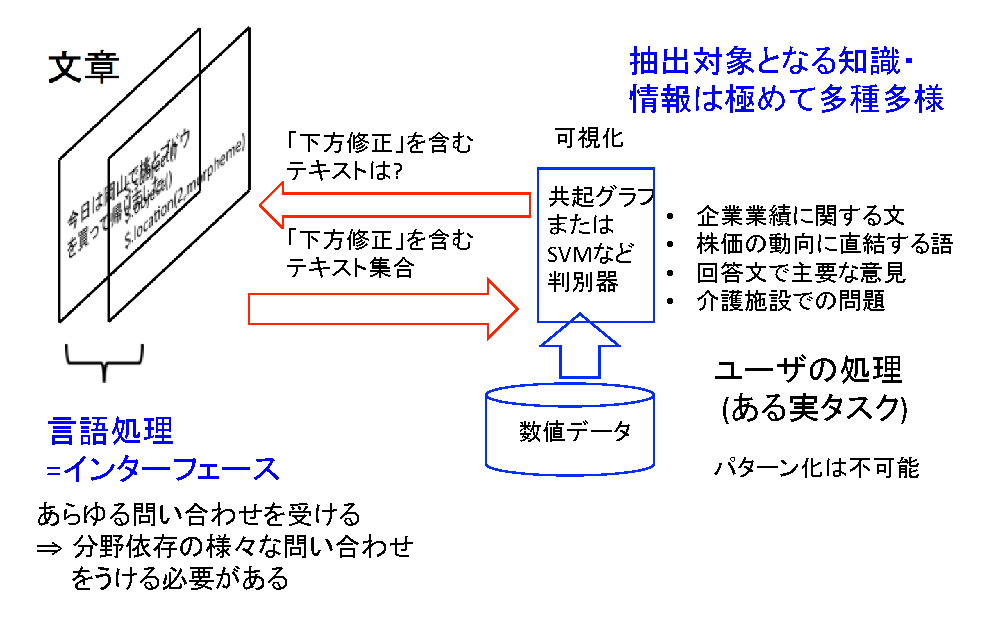
\includegraphics[scale=0.4]{fig/lang.eps}
\end{center}
\caption {言語処理は文書に対するあらゆる問い合わせを受けるインターフェース}
\label{fig:lang}
\end{figure}


\section{言語処理の位置付けと発展}
上記で取り上げたテキストマイニングに関する研究は処理に主眼があるわけではなく,取り出した
テキストに価値があることが明らかである.一方で,言語処理はテキストから必要な情報(それは
分野依存であり,前もって分野非依存で用意することが不可能な情報)を取り出すための
ありとあらゆるテキストに対する操作が要求される部分であるということである.
例えば,企業情報であれば,「企業活動を表す文書」を集める必要があり,文の中では「企業名」
やその「活動 」表現する部分を獲得し,表現の正規化が必要になる.それらをこなすツールは
存在しないため,「企業活動を表す文書」を表すには,そうした記事を書いてるニュースサイト
を固定したり,「活動」などはキーワードを決めるか「動詞」といった品詞レベルで押さえる
といった手法しかない.よって問題・分野に依存した,テキスト情報抽出手法の開発は
有益である.
さらに,テキストマイニングの主は価値ある情報であり,分析者はツール構築に興味は無い.
この部分において,言語処理を研究している研究者が分析者と共同で活動することで
より具体的な実処理に役立つ研究テーマと成果が得られるのではないかと推察できる.


\bibliographystyle{jplain}
\bibliography{all,my-results}
\end{document} 

